\documentclass[aps,prl,twocolumn,showpacs,superscriptaddress,groupedaddress]{revtex4}  % for review and submission
%\documentclass[aps,prl,preprint,groupedaddress]{revtex4-1}

%\documentclass[aps,preprint,showpacs,superscriptaddress,groupedaddress]{revtex4}  % for double-spaced preprint
\usepackage{graphicx}  % needed for figures
\usepackage{dcolumn}   % needed for some tables
\usepackage{bm}        % for math
\usepackage{amssymb}   % for math

% avoids incorrect hyphenation, added Nov/08 by SSR
%hyphenation{ALPGEN}

\begin{document}

% The following information is for internal review, please remove them for submission
\widetext
\leftline{Version xx as of \today}
\leftline{Primary authors: MIT, NTU}
\leftline{To be submitted to PRL}

\title{Measurements of two-particle correlations in $e^+e^-$ collisions at 91 GeV with ALEPH archived data}
\author{Yen-Jie Lee}
\author{Gian Michele Innocenti}
\author{Austin Baty}
\author{Chris McGinn}
\author{Anthony Badea}
\affiliation{Massachusetts Institute of Technology}%
\author{Paoti Chang}
\author{Tzu-An Sheng}
\author{Bean Huang}
\affiliation{National Taiwan University}%
\author{Marcello Maggi}
\affiliation{INFN Bari}%
\date{\today}


\begin{abstract}
The first measurement of two-particle angular correlations for charged particles emitted in $e^+e^-$ collisions at center-of-mass energy of 91 GeV are presented. The archived data are collected with the ALEPH detector at LEP. The correlation functions are measured over a broad range of pseudorapidity and azimuthal angle of the charged particles. Those results are compared to predictions from PYTHIA event generator. In contrast to the results from high charged particle multiplicity nuleon-nucleon, nucleon-nucleus and nuclenus-nucleus collisions, where long-range correlations with large pseudorapidity gap are observed, no significant enhancement of long-range correlations is observed with respect to PYTHIA predictions, which do not include additional final state interactions. This reference measurement shows the observed long-range correlations in RHIC and LHC are coming from either initial state correlations in the nucleons and nucleus, or final state interaction of the outgoing partons
\end{abstract}

\pacs{}
\maketitle

%%%%%%%%%%%%%%%%%%%%%%%%%%%%%%%%%%%%%%%%%%%%%%%%%%%%%%%%%%%%%%%%%%%%%%%%%%%%%
\section{\label{sec:introduction}Introduction}
Two-particle correlations in high-energy collisions provide valuable information for characterizing Quantum Chromodynamics and have been studied previously for a broad range of collision energies in proton-proton (pp)~\cite{Khachatryan:2010gv}, proton-nucleus (pA)~\cite{CMS:2012qk,Abelev:2012ola,Aad:2012gla}, deutron-nucleus (dA)~\cite{}, and nucleus-nucleus (AA)~\cite{Aamodt:2010pa,Chatrchyan:2012wg} collisions. Such measurements can elucidate the underlying mechanism of particle production and reveal possible collective effects resulting from the high particle densities accessible in these collisions.
Studies of two-particle angular correlations are typically performed using two-dimensional $\Delta\eta-\Delta\phi$ correlation functions, where $\Delta\phi$ is the difference in the azimuthal angle $\phi$ between the two particles and $\Delta\eta$ is the difference in pseudorapidity $\eta = -\ln(\tan(\theta/2))$. The polar angle $\theta$ is defined relative to the counterclockwise hadron beam direction.
Of particular interest in studies of collective effects is the long-range (large $|\Delta\eta|$) structure of the two-particle correlation functions. In this region, the function is less susceptible to other known sources of correlations such as resonance decays and fragmentation function of energetic jets. Measurements in high-energy AA collisions have shown significant modification of the long-range structure compared with minimum-bias pp collisions, over a very wide range of collision energies~\cite{Back:2004je,Arsene:2004fa,Adcox:2004mh,Adams:2005dq}. The long-range correlations are interpreted as a consequence of the hydrodynamical flow of the produced strongly interacting medium~\cite{Ollitrault:1992bk} and usually characterized by the Fourier components of the azimuthal particle distributions. The extraction of the second and third Fourier components, usually referred to as elliptic and triangular flow, is of great interest because it is closely related to initial collision geometry and its fluctuation~\cite{Alver:2010gr}. Those measurements allow the extraction of the fundamental transport properties of the medium using hydrodynamic models.
Recently, measurements in pp~\cite{Khachatryan:2010gv}, pPb collisions~\cite{CMS:2012qk,Abelev:2012ola,Aad:2012gla} and dAu collisions~\cite{} have revealed the emergence of long-range, near-side ($\Delta\phi\sim 0$) correlations in the selection of collisions with very high number of final state particles. This long-range correlation has inspired a large variety of theoretical models~\cite{Bzdak:2013zma,Dusling:2015gta}. The physical origin of the phenomenon is not yet fully understood. Moreover, it was found that the elliptic flow signal exists even at the lowest nucleon-nucleon center-of-mass energy of 7.7 GeV in AA collisions at the Relativistic Heavy Ion Collider~\cite{Adamczyk:2012ku}. 
Due to the complexity of the hadron-hadron collisions, possible initial state correlations of the partons, such as those arise from color-glass condensate~\cite{Gelis:2010nm, Dusling:2013qoz}, could complicate the interpretation of the pp and pA data. Studies of high charged particle multiplicity $e^+e^-$ collision, where the initial kinematics of the collisions are well-defined, could bring significant insights about the observed phenomenon. 
%These measurements will also enable a direct comparison between different collision systems for the first time. 
The studies of ridge signal in $e^+e^-$ collisions will bring significant impact to the field of relativistic heavy ion collisions, either change completely the interpretation of the ridge in pp, pA and AA collisions if a significant signal is observed, or serve as an important reference for the initial state and final state effect observed in high multiplicity hadron-hadron scatterings if no long-range correlation signal was detected. 

In this paper, ..


\begin{figure}[!htb]
\begin{center}
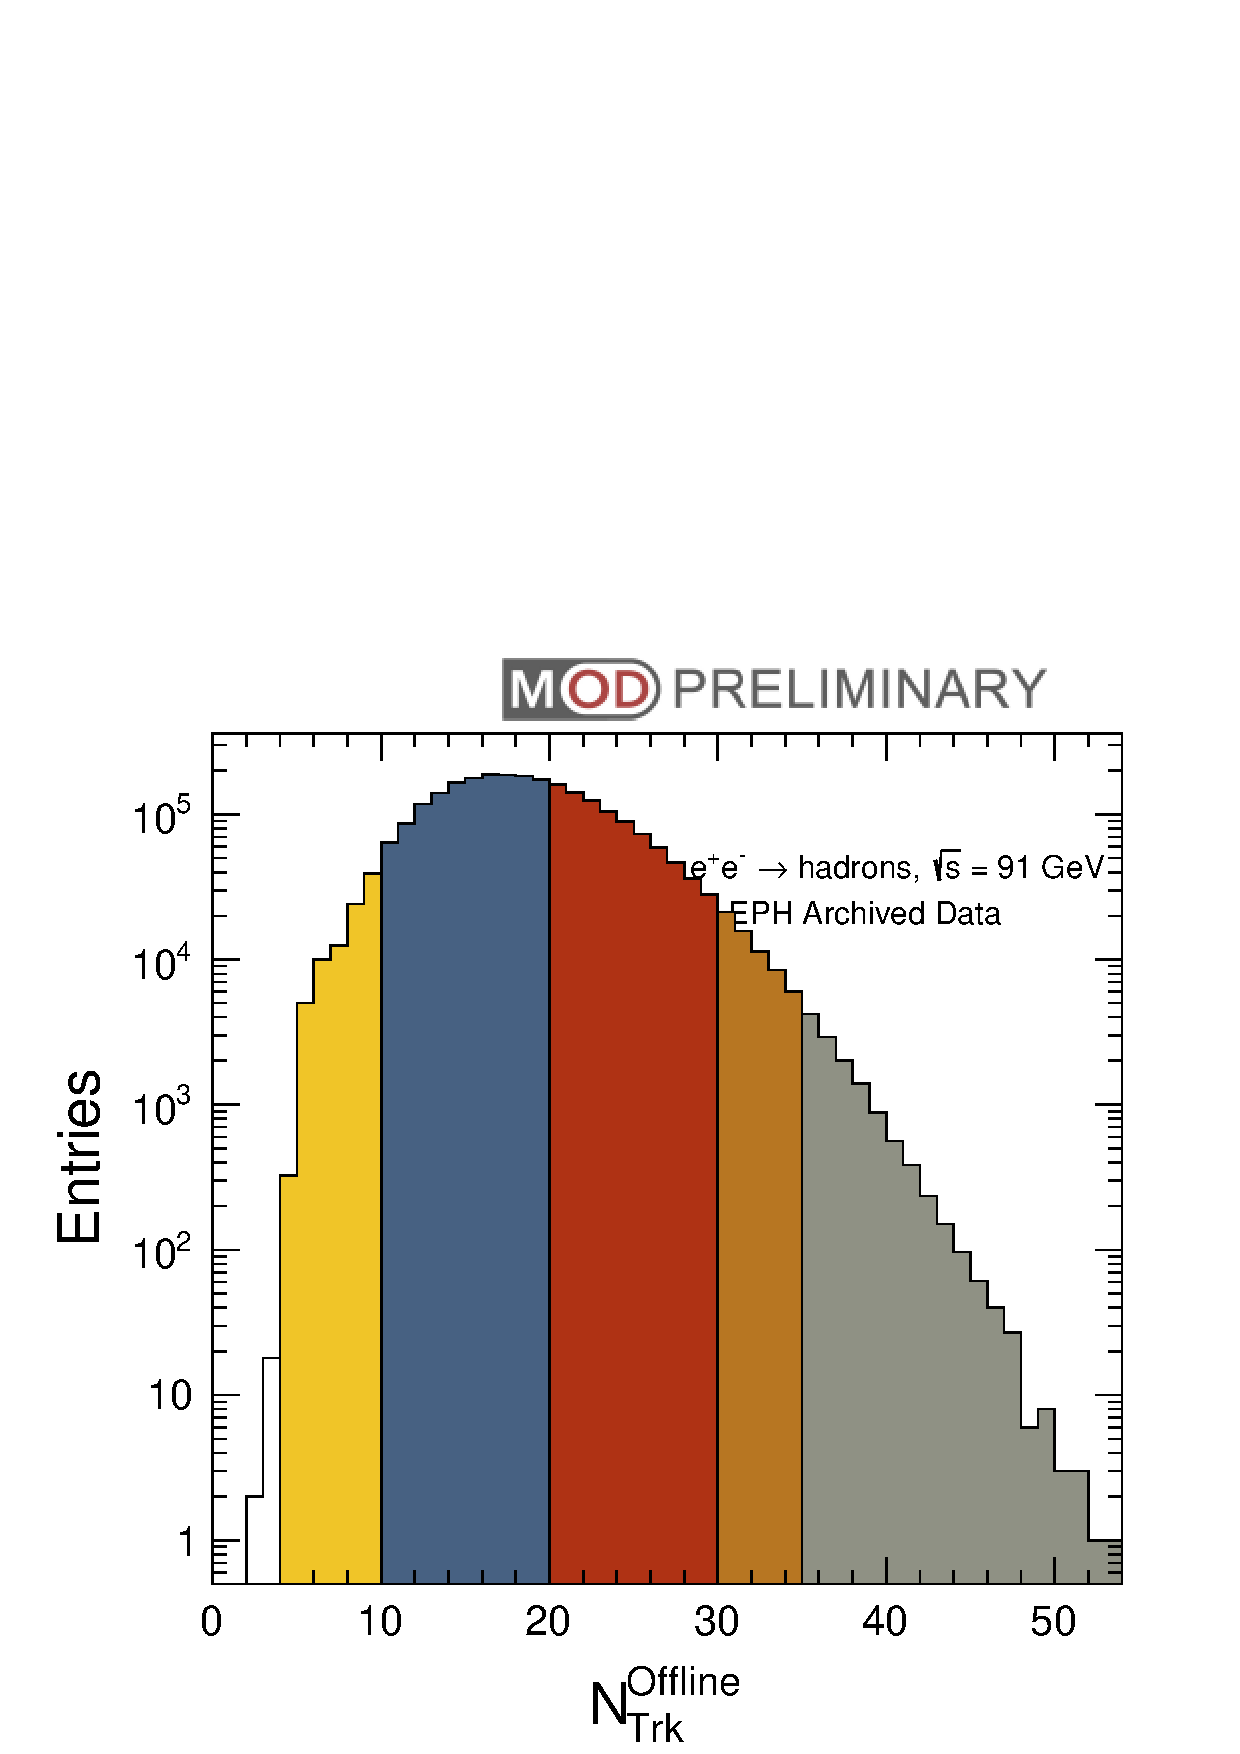
\includegraphics[width=.45\textwidth]{plots/event/nTrkOffline.png}
\caption{Charged particle multiplicity in ALEPH archived data}
\label{fig:figure1} 
\end{center}
\end{figure}


%%%%%%%%%%%%%%%%%%%%%%%%%%%%%%%%%%%%%%%%%%%%%%%%%%%%%%%%%%%%%%%%%%%%%%%%%%%%%
\section{\label{sec:datasample}Data Sample and Event Selection}

\subsection{\label{sec:}ALEPH Detector}
\subsection{\label{sec:}Event Selection}
\subsection{\label{sec:}Data Sample and Detector Corrections}

%%%%%%%%%%%%%%%%%%%%%%%%%%%%%%%%%%%%%%%%%%%%%%%%%%%%%%%%%%%%%%%%%%%%%%%%%%%%%
\section{\label{sec:analysis}Analysis Technique}
In this analysis, identified protons, pions and kaons with transverse momentum between 0.1 and 4.0 GeV/$c$ 
are selected for the correlation function analysis. High multiplicity events are sampled using the total number of selected proton, 
pions and kaons (hadron multiplicity $N$) in each event. The first step in extracting the correlation function was to divide the sample 
into bins in the hadron multiplicity. For each hadron multiplicity class, ``trigger" particles are defined as charged hadrons in the selected transverse momentum range (0.1 and 4.0 GeV/$c$). Particle pairs are then formed by associating every trigger particle with the remaining charged hadrons in the same $p_{\rm T}$ interval as the trigger particle. The per-trigger-particle associated yield is defined as:
\begin{eqnarray}
\label{eq:associatedyield}
\frac{1}{N_{\rm trig}}\frac{\rm d^2N^{pair}}{d\Delta\eta  \rm d\Delta\phi}= B(0,0) \times \frac{S(\Delta\eta, \Delta\phi)}{B(\Delta\eta, \Delta\phi)}
\end{eqnarray}
where $N_{trig}$ is the number of trigger particles in the event, $\Delta\eta$ and $\Delta\phi$ are the differences in $\eta$ and $\phi$ of the pair. The signal distribution, $S(\Delta\eta, \Delta\phi)$, 
is the per-trigger-particle yield of particle pairs in the same event: 
\begin{eqnarray}
\label{eq:S}
S(\Delta\eta,\Delta\phi) = \frac{1}{N_{trig}}\frac{\rm d^2 N^{\rm same}}{\rm d\Delta\eta \rm d\Delta\phi}
\end{eqnarray}
The mixed-event background distribution, used to account for random combinatorial background, is defined as 
\begin{eqnarray}
\label{eq:B}
B(\Delta\eta,\Delta\phi) = \frac{1}{N_{trig}}\frac{\rm d^2 N^{\rm mix}}{\rm d\Delta\eta \rm d\Delta\phi}
\end{eqnarray}
and is constructing by pairing the trigger particles from two random events in the same hadron multiplicity interval.
The symbol $N^{mix}$ denotes the number of pairs taken from the mixed event, while $B(0,0)$ represents the mixed-event associated yield for both particles of the pair going in the same direction and thus having full pair acceptance. Therefore, 
the ratio $B(0,0)/B(\Delta\eta,\Delta\phi)$ represents the pair-acceptance correction factor used to derive the corrected per-trigger-particle
associated yield distribution.  The signal and background distributions are first calculated for each event and then averaged over all the events within the track multiplicity class. 

%%%%%%%%%%%%%%%%%%%%%%%%%%%%%%%%%%%%%%%%%%%%%%%%%%%%%%%%%%%%%%%%%%%%%%%%%%%%%
\section{\label{sec:results}Results}
In Fig.~\ref{fig:figure1}, the two-particle correlation functions from low (N$>$20) multiplicity events is presented. In low-multiplicity events, the dominant features of the correlation function are the jet peak near $(\Delta\eta,\Delta\phi)=(0,0)$ for pairs of particles originating from the same jet and the elongated structure at $\Delta\phi\sim\pi$ for pairs of particles from back-to-back jets. %To better illustrate the full correlation structure, the jet peak has been truncated in the high multiplicity event.
The same-side jet peak and back-to-back correlation structures are also observed in high multiplicity events. 
In addition, a hint of ``ridge"-like structure is visible at $\Delta\phi \sim$0 in the right panel of Fig.~\ref{fig:figure2}. 
%To separate and inspect the long-range and short-range structure, one-dimensional distributions in $\Delta\phi$ are obtained by integrating over two $|\Delta\eta|$ intervals: 0$<|\Delta \eta|<$1 and 
%2$<|\Delta \eta|<$3.  At small $\Delta\eta$, a near-side peak at $\Delta\phi=$0 and the contribution from the back-to-back jet at $\Delta\phi=\pi$ is observed in the left panel of Fig~\ref{fig:figure1}. At large $\Delta\eta$, a near-side peak at $\Delta\phi=0$ is shown in the right panel of Fig~\ref{fig:figure1}, similar to the structures observed in high multiplicity pp, pA and AA collisions over a wide range of energies. However, the significance of this signal is limited by the available statistics.

\begin{figure}[!htb]
\begin{center}
\includegraphics[width=.23\textwidth]{plots/beam/beamAxisAnalysis.png}
\includegraphics[width=.23\textwidth]{plots/beam/beamAxisAnalysisProjection.png}
\caption{Two-particle correlation functions versus $\Delta\eta$ and $\Delta\phi$ in $e^{+}e^{-}$ collisions for events with particle multiplicity $>$ 35 with beam axis.}
\label{fig:figure1} 
\end{center}
\end{figure}

\begin{figure}[!htb]
\begin{center}
\includegraphics[width=.23\textwidth]{plots/thrust/thrustAxisAnalysis.png}
\includegraphics[width=.23\textwidth]{plots/thrust/thrustAxisAnalysisProjection.png}
\caption{Two-particle correlation functions versus $\Delta\eta$ and $\Delta\phi$ in $e^{+}e^{-}$ collisions for events with particle multiplicity $>$ 35 with thrust axis.}
\label{fig:figure1} 
\end{center}
\end{figure}

\begin{figure}[!htb]
\begin{center}
\includegraphics[width=.23\textwidth]{plots/thrustBarrel/thrustAxisBarrelAnalysis.png}
\includegraphics[width=.23\textwidth]{plots/thrustBarrel/thrustAxisBarrelAnalysisProjection.png}
\caption{Two-particle correlation functions versus $\Delta\eta$ and $\Delta\phi$ in $e^{+}e^{-}$ collisions for events with particle multiplicity $>$ 30 with thrust axis with barrel selection.}
\label{fig:figure1} 
\end{center}
\end{figure}



%%%%%%%%%%%%%%%%%%%%%%%%%%%%%%%%%%%%%%%%%%%%%%%%%%%%%%%%%%%%%%%%%%%%%%%%%%%%%
\section{\label{sec:systematic}Systematic uncertainties}
Add here discussion of the systematic results

%%%%%%%%%%%%%%%%%%%%%%%%%%%%%%%%%%%%%%%%%%%%%%%%%%%%%%%%%%%%%%%%%%%%%%%%%%%%%
\section{\label{sec:monteCarlo}Monte carlo comparison}
Add here discussion of the monte carlo comparisons

\subsection{\label{sec:LEP2}LEP2}


%%%%%%%%%%%%%%%%%%%%%%%%%%%%%%%%%%%%%%%%%%%%%%%%%%%%%%%%%%%%%%%%%%%%%%%%%%%%%
\section{\label{sec:summary}Summary}
The ALEPH data has been used to perform measurements of two-particle angular correlation functions for the first time. A hint of long-range ($|\Delta\eta|>2$) ridge-like structure at the
near-side ($\Delta\phi\sim 0$) was shown in the Belle data. However, the limited statistics precludes drawing firm conclusions and we propose to perform those measurements with the unique high statistics hadronic data recorded by the Belle detector.


%%%%%%%%%%%%%%%%%%%%%%%%%%%%%%%%%%%%%%%%%%%%%%%%%%%%%%%%%%%%%%%%%%%%%%%%%%%%%
\section{\label{sec:datasample}Global Observables}
%%%%%%%%%%%%%%%%%%%%%%%%%%%%%%%%%%%%%%%
%%%%%%%%%%%%%%%%%%%%%%%%%%%%%%%%%%%%%%%
\subsection{LEP2 Monte-Carlo}
%%%%%%%%%%%%%%%%%%%%%%%%%%%%%%%%%%%%%%%

%%%%%%%%%%%%%%%%%%%%%%%%%%%%%%%%%%%%%%%%%%%%%%%%%%%%%%%%%%%%%%%%%%%%%%%%%%%%% 
\begin{acknowledgments}
We wish to acknowledge ......
\dots.
\end{acknowledgments}

\nocite{*}
\bibliography{ridgepaperALEPH}

\end{document}
%
% ****** End of file template.aps ******
